%!TEX TS-program = xelatex
%!TEX encoding = UTF-8 Unicode

\documentclass[11pt,tikz,border=1]{standalone}

\begin{document}
  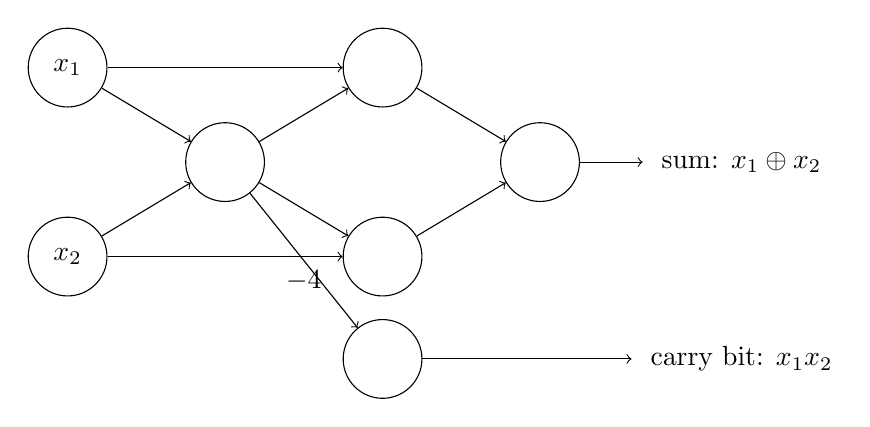
\begin{tikzpicture}[
    neuron/.style={circle,draw,inner sep=0pt,minimum size=10mm}
    ]

    \node (x1) at (-6, 1.2) [neuron] {$x_1$};
    \node (x2) at (-6, -1.2) [neuron] {$x_2$};
    \node (pl1) at (-4, 0) [neuron] {};
    \node (pm1) at (-2, 1.2) [neuron] {};
    \node (pm2) at (-2, -1.2) [neuron] {};
    \node (pm3) at (-2, -2.5) [neuron] {};
    \node (pr1) at (0, 0) [neuron] {};
    \node (sum) at (2.5, 0) {\ sum: $x_1 \oplus x_2$};
    \node (carrybit) at (2.5, -2.5) {\ carry bit: $x_1x_2$};
    \draw [->] (x1) to (pl1);
    \draw [->] (x2) to (pl1);
    \draw [->] (x1) to (pm1);
    \draw [->] (x2) to (pm2);
    \draw [->] (pl1) to (pm1);
    \draw [->] (pl1) to (pm2);
    \draw [->] (pl1) to node [below] {$-4$} (pm3);
    \draw [->] (pm1) to (pr1);
    \draw [->] (pm2) to (pr1);
    \draw [->] (pr1) to (sum);
    \draw [->] (pm3) to (carrybit);

  \end{tikzpicture} 
\end{document}
